\documentclass[8pt,landscape]{article}

% PACKAGES
\usepackage[letterpaper, margin=0.1in]{geometry}
\usepackage{amsmath, amssymb}
\usepackage{multicol}
\usepackage{setspace}
\usepackage{sectsty}
\usepackage{verbatim}
\usepackage{graphicx}
\usepackage{xcolor}
\usepackage{listings}
\usepackage{xcolor}
\usepackage{enumitem}

\setlist{nosep, leftmargin=*}
\lstset{
  basicstyle=\ttfamily\footnotesize,
  backgroundcolor=\color{gray!10},
  frame=single,
  breaklines=true,
  columns=fullflexible,
  showstringspaces=false,
  keywordstyle=\color{blue},
  commentstyle=\color{gray},
  stringstyle=\color{orange}
}
% FORMATTING
\setstretch{0.9}
\setlength{\parindent}{0pt}
\setlength{\parskip}{0pt}

% Reduce subsection spacing and make subsections blue
\makeatletter
\renewcommand{\section}{\@startsection{section}{2}{0pt}%
    {0.2ex}% space before subsection
    {0.2ex}% space after subsection
    {\fontsize{8}{8}\bfseries\color{red}}} % font size, bold, blue color
\makeatother

% Reduce subsection spacing and make subsections blue
\makeatletter
\renewcommand{\subsection}{\@startsection{subsection}{2}{0pt}%
    {0.2ex}% space before subsection
    {0.2ex}% space after subsection
    {\fontsize{8}{8}\bfseries\color{blue}}} % font size, bold, blue color
\makeatother
% Custom small text wrapper
\newcommand{\smalltext}[1]{%
  {\fontsize{8}{7}\selectfont\sloppy #1\par}%
}

% DOCUMENT START
\begin{document}
\pagestyle{empty}
\begin{multicols}{3}
\subsection*{The Central Limit Theorem (CLT)}
\smalltext{
\begin{itemize}
    \item The sampling distribution is centered around the true population mean.
    \item As the sample size increases, most sample means cluster closely around the true mean.
    \item The sampling distribution’s shape may differ from the population’s distribution but becomes more symmetrical and bell-shaped with larger samples.
    \item Both the figures and plots clearly demonstrate the Central Limit Theorem.
\end{itemize}
Regardless of the parent population distribution whose mean is $\mu$ and standard deviation is $\sigma$, 
the Central Limit Theorem (CLT) states that the sampling distribution of the sample mean $\bar{X}$ 
converges to a Normal distribution with mean $\mu$ and standard deviation $\dfrac{\sigma}{\sqrt{n}}$ 
as the sample size $n$ increases, when sampling with replacement.
The above CLT conditions can be mathematically defined as:
\[
\bar{X} \sim \mathcal{N}\left(\mu, \frac{\sigma}{\sqrt{n}}\right)
\quad \text{as} \quad n \to \infty
\]
\subsection{Confidence Interval for Continuous Cases}
Note we need to define \textbf{SE}:
\[
\text{Confidence Interval} = \text{Point Estimate} \pm 
\underbrace{Z_{1-\alpha/2} \times \text{SE}}_{\text{MoE}}
\]
From the CLT definition, the \textbf{standard error} would be:
\[
\text{SE} = \frac{\hat{\sigma}}{\sqrt{n}}
\]
}
\begin{lstlisting}[language=R]
#Calculate proportions
click_through %>%
  group_by(webpage) %>%
  summarize(
    prop = sum(click_target) / n(),
    successes = prop * n(),
    failures = n() * (1 - prop)
  )
#Calculate Standard Error
click_through_est <- click_through %>%
  group_by(webpage) %>%
  summarize(
    click_rate = sum(click_target) / n(),
    n = n()
  ) %>%
  mutate(se = sqrt(click_rate * (1 - click_rate) / n))
#Calculate Confidence Intervals
click_through_CLT_95_ci <- click_through_est %>%
  mutate(
    lower_95 = click_rate - (qnorm(0.975) * se), #for 90CI qnorm(0.95)
    upper_95 = click_rate + (qnorm(0.975) * se), #for 90CI qnorm(0.95)
    Method = rep("CLT", 2)
  )
\end{lstlisting}
\subsection{Dif between CI from CLT and bootstrapped}
\smalltext{
CLT  we are finding the CI directly from the sample.
Bootstrapped (empirical) and CLT (theoritical) give almost same CI results for a sufficiently large sample. 
}
\subsection{When to use CLT or bootstrapped}
\smalltext{
If computational speed does not matter, and you do not violate any of the conditions of the CLT, then you can either use a simulation-based approach (like bootstrapping) or CLT, and you will get essentially the same results.
If you are violating the conditions of the CLT, then you might want to use simulation-based approaches. 
}
\subsection{Hypothesis tests based on normal and t-distributions}
\smalltext{
\begin{itemize}
    \item a Normal distribution when we are testing for a difference in proportions;
    \item t-distribution when we are testing for a difference of continuous means.
\end{itemize}
}
\subsection{Proportions}
\begin{lstlisting}[language=R]
#Shortcut for tests in proportions case
click_summary <- click_through %>%
  group_by(webpage) %>%
  summarize(
    success = sum(click_target),
    n = n()
  )
prop.test(x = click_summary$success, n = click_summary$n,
  correct = FALSE, alternative = "less"
)
\end{lstlisting}
\smalltext{
The square of a z-score is almost equal to Chi-square test.
If p-value  $ < \alpha$, then we have enough statistical evidence to reject the null hypothesis in favour of the alternative hypothesis.
}

\section{Continuous}
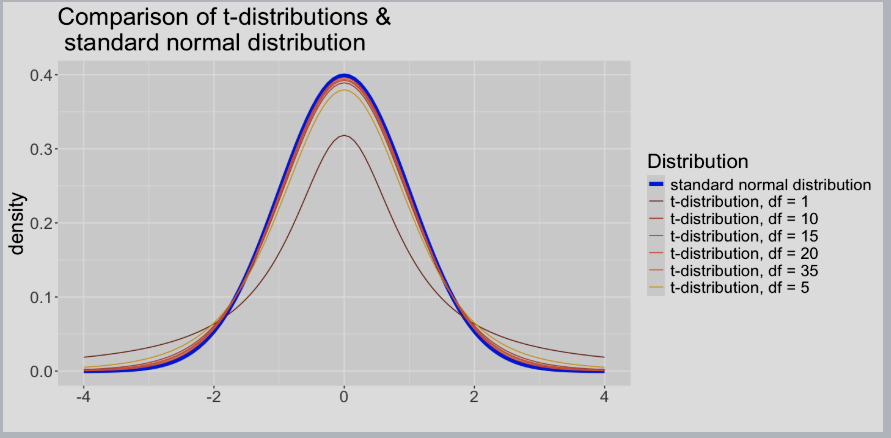
\includegraphics[width=0.9\linewidth]{t-test.png}
\subsection{One-sample t-test}
\subsection{two-sample t-test}
\begin{lstlisting}[language=R]
#Shortcut for tests in continuous case
twospecies_data <- penguins |>
  filter(species %in% c("Adelie", "Gentoo")) |>
  drop_na(flipper_length_mm)
# Perform the t-test
t_test_result <- t.test(flipper_length_mm ~ species, data = twospecies_data, alternative = "less")
\end{lstlisting}
\section{Deciding Which Test to Use}
\smalltext{
The choice of statistical test depends primarily on the type of variables being compared and the research question:
\subsection{Chi-Square Tests ($\chi^2$) : Categorical Variables}  
If your analysis involves comparing observed counts to expected counts for one or more categorical variables, you should use \textbf{Chi-Square Tests}. \\
The main assumptions of Chi-squared tests are that:\\
The observations are independent.\\
The expected counts are sufficiently large (greater than 5 is the typical standard). \\
The notion of chi-squared tests is to compare observed counts with expected counts from a population or distribution. In general, the hypotheses can be formulated as: \\
$H_O$: The observed ($O$) and expected ($E$) counts are equal. \\
$H_A$: The observed ($O$) and expected ($E$) counts are not equal. \\
\textbf{One Categorical Variable:} \\
- Use the \textit{Chi-Square Goodness of Fit Test} to see if the distribution of that single variable matches a hypothesized distribution (e.g., equal distribution).
}
\begin{lstlisting}[language=R]
observed <- mm$Count
expected <- rep(sum(mm$Count) / 6, 6)
X_sq <- sum((observed - expected)^2 / expected) # Chi-Square 
pchisq(X_sq, df=8, lower.tail=FALSE) # p-value 
chi_test_result <- chisq.test(x = mm$Count, correct = FALSE) #To get all the chi test values
chi_test_result <- chi_test_result$statistic
\end{lstlisting}
\smalltext{
\textbf{Two Categorical Variables:}  \\
- Use the \textit{Chi-Square Test of Independence/Homogeneity} to determine if the distribution of one variable depends on the other (e.g., is click-through rate independent of the webpage version?).  
\\
\textit{Note:} When comparing two categories, this test is mathematically equivalent to a two-sample proportion test.
}
\begin{lstlisting}[language=R]
count_table_AB <- click_through |>
  tabyl(webpage, click_target)
chisq.test(cont_table_AB, correct = FALSE)
\end{lstlisting}
\smalltext{

\subsection{One-Way Analysis of Variance (ANOVA): Continuous Variables}  
If you want to compare the means of a continuous outcome across the levels of a single categorical factor, use \textbf{Analysis of Variance (ANOVA)}. \\
\textbf{ANOVA Hypotheses:}  \\
- Use this if the assumptions of \textit{Normality (of residuals)} and \textit{Equal Variance} across groups are met. \\
$H_O$: All means are equal $(\mu_1 = \mu_2 = .... = \mu_k)$ \\
$H_A$: Not all means are equal. \\
}
\begin{lstlisting}[language=R]
res <- aov(flipper_length_mm ~ species, data = penguins)
summary(res)
p_value <- summary(res)[[1]]$'Pr(>F)'[1]
\end{lstlisting}
\smalltext{
\textbf{The $F$-test:}  \\
- The test statistic is an $F$-ratio that compares the variance between groups (Treatment Sum of Squares, $\text{SST}$) to the variance within groups \\
}

\subsection{ANOVA Assumptions}  
\smalltext{
\textbf{Normality:} Residuals should be approximately normally distributed (checked via Q-Q plots or Shapiro-Wilk test). \\
\textbf{Equal Variance (Homoscedasticity):} Population variances should be equal across groups (checked via Levene's test). \\
\textbf{Independent Observations.} \\
}

\begin{lstlisting}[language=R]
shapiro.test(res$residuals)
leveneTest(flipper_length_mm ~ species, data = penguins)
\end{lstlisting}

\subsection{Nonparametric Alternative: Kruskal-Wallis Test}  
\smalltext{
When the normality assumption is violated, the Kruskal-Wallis Test serves as a robust alternative, comparing group medians based on the ranks of the data rather than the raw values. \\
When comparing two groups in ANOVA, the $p$-value matches the two-sample $t$-test, and the $F$-statistic equals the square of the $t$-statistic ($\text{F} \approx t^2$). \\ 
When comparing two categories in the $\chi^2$ test for independence, the test statistic and $p$-value match the two-sample proportion test.\\
}


\end{multicols}
\end{document}